% Template for a Computer Science Tripos Part II project dissertation
\documentclass[12pt,a4paper,twoside,openright]{report}
\usepackage[pdfborder={0 0 0}]{hyperref}    % turns references into hyperlinks
\usepackage[margin=25mm]{geometry}  % adjusts page layout
\usepackage{graphicx}  % allows inclusion of PDF, PNG and JPG images
\usepackage{verbatim}
\usepackage{docmute}   % only needed to allow inclusion of proposal.tex

\raggedbottom                           % try to avoid widows and orphans
\sloppy
\clubpenalty1000%
\widowpenalty1000%

\renewcommand{\baselinestretch}{1.1}    % adjust line spacing to make
                                        % more readable

\begin{document}

\bibliographystyle{plain}


%%%%%%%%%%%%%%%%%%%%%%%%%%%%%%%%%%%%%%%%%%%%%%%%%%%%%%%%%%%%%%%%%%%%%%%%
% Title


\pagestyle{empty}

\rightline{\LARGE \textbf{Martin Richards}}

\vspace*{60mm}
\begin{center}
\Huge
\textbf{How to write a dissertation in \LaTeX} \\[5mm]
Computer Science Tripos -- Part II \\[5mm]
St John's College \\[5mm]
\today  % today's date
\end{center}

%%%%%%%%%%%%%%%%%%%%%%%%%%%%%%%%%%%%%%%%%%%%%%%%%%%%%%%%%%%%%%%%%%%%%%%%%%%%%%
% Proforma, table of contents and list of figures

\pagestyle{plain}

\chapter*{Proforma}

{\large
\begin{tabular}{ll}
Name:               & \bf Martin Richards                       \\
College:            & \bf St John's College                     \\
Project Title:      & \bf How to write a dissertation in \LaTeX \\
Examination:        & \bf Computer Science Tripos -- Part II, July 2001  \\
Word Count:         & \bf 1587\footnotemark[1]
                      (well less than the 12000 limit)  \\
Project Originator: & Dr M.~Richards                    \\
Supervisor:         & Dr Markus Kuhn                    \\ 
\end{tabular}
}
\footnotetext[1]{This word count was computed
by \texttt{detex diss.tex | tr -cd '0-9A-Za-z $\tt\backslash$n' | wc -w}
}
\stepcounter{footnote}


\section*{Original Aims of the Project}

To write a demonstration dissertation\footnote{A normal footnote without the
complication of being in a table.} using \LaTeX\ to save
student's time when writing their own dissertations. The dissertation
should illustrate how to use the more common \LaTeX\ constructs. It
should include pictures and diagrams to show how these can be
incorporated into the dissertation.  It should contain the entire
\LaTeX\ source of the dissertation and the makefile.  It should
explain how to construct an MSDOS disk of the dissertation in
Postscript format that can be used by the book shop for printing, and,
finally, it should have the prescribed layout and format of a diploma
dissertation.


\section*{Work Completed}

All that has been completed appears in this dissertation.

\section*{Special Difficulties}

Learning how to incorporate encapulated postscript into a \LaTeX\
document on both Ubuntu Linux and OS X.
 
\newpage
\section*{Declaration}

I, [Name] of [College], being a candidate for Part II of the Computer
Science Tripos [or the Diploma in Computer Science], hereby declare
that this dissertation and the work described in it are my own work,
unaided except as may be specified below, and that the dissertation
does not contain material that has already been used to any substantial
extent for a comparable purpose.

\bigskip
\leftline{Signed [signature]}

\medskip
\leftline{Date [date]}

\tableofcontents

\listoffigures

\newpage
\section*{Acknowledgements}

This document owes much to an earlier version written by Simon Moore
\cite{Moore95}.  His help, encouragement and advice was greatly 
appreciated.

%%%%%%%%%%%%%%%%%%%%%%%%%%%%%%%%%%%%%%%%%%%%%%%%%%%%%%%%%%%%%%%%%%%%%%%
% now for the chapters

\pagestyle{headings}

\chapter{Introduction}

\section{Overview of the files}

This document consists of the following files:

\begin{itemize}
\item \texttt{makefile} --- The makefile for the dissertation and
                         Project Proposal
\item \texttt{diss.tex} --- The dissertation
\item \texttt{proposal.tex}  --- The project proposal 
\item \texttt{figs} -- A directory containing diagrams and pictures
\item \texttt{refs.bib} --- The bibliography database
\end{itemize}

\section{Building the document}

This document was produced using \LaTeXe which is based upon
\LaTeX\cite{Lamport86}.  To build the document you first need to
generate \texttt{diss.aux} which, amongst other things, contains the
references used.  This if done by executing the command:

\texttt{pdflatex diss}

\noindent
Then the bibliography can be generated from \texttt{refs.bib} using:

\texttt{bibtex diss}

\noindent
Finally, to ensure all the page numbering is correct run \texttt{pdflatex}
on \texttt{diss.tex} until the \texttt{.aux} files do not change.  This
usually takes 2 more runs.

\subsection{The makefile}

To simplify the calls to \texttt{pdflatex} and \texttt{bibtex}, 
a makefile has been provided, see Appendix~\ref{makefile}. 
It provides the following facilities:

\begin{description}

\item\texttt{make} \\
 Display help information.

\item\texttt{make proposal.pdf} \\
 Format the proposal document as a PDF.

\item\texttt{make view-proposal} \\
 Run \texttt{make proposal.pdf} and then display it with a Linux PDF viewer
 (preferably ``okular'', if that is not available fall back to ``evince'').

\item\texttt{make diss.pdf} \\
 Format the dissertation document as a PDF.

\item\texttt{make count} \\
Display an estimate of the word count.

\item\texttt{make all} \\
Construct \texttt{proposal.pdf} and \texttt{diss.pdf}.

\item\texttt{make pub} \\ Make \texttt{diss.pdf}
and place it in my \texttt{public\_html} directory.

\item\texttt{make clean} \\ Delete all intermediate files except the
source files and the resulting PDFs. All these deleted files can
be reconstructed by typing \texttt{make all}.

\end{description}


\section{Counting words}

An approximate word count of the body of the dissertation may be
obtained using:

\texttt{wc diss.tex}

\noindent
Alternatively, try something like:

\verb/detex diss.tex | tr -cd '0-9A-Z a-z\n' | wc -w/


\chapter{Preparation}

This chapter is empty!


\chapter{Implementation}

\section{Verbatim text}

Verbatim text can be included using \verb|\begin{verbatim}| and
\verb|\end{verbatim}|. I normally use a slightly smaller font and
often squeeze the lines a little closer together, as in:

{\renewcommand{\baselinestretch}{0.8}\small
\begin{verbatim}
GET "libhdr"
 
GLOBAL { count:200; all  }
 
LET try(ld, row, rd) BE TEST row=all
                        THEN count := count + 1
                        ELSE { LET poss = all & ~(ld | row | rd)
                               UNTIL poss=0 DO
                               { LET p = poss & -poss
                                 poss := poss - p
                                 try(ld+p << 1, row+p, rd+p >> 1)
                               }
                             }
LET start() = VALOF
{ all := 1
  FOR i = 1 TO 12 DO
  { count := 0
    try(0, 0, 0)
    writef("Number of solutions to %i2-queens is %i5*n", i, count)
    all := 2*all + 1
  }
  RESULTIS 0
}
\end{verbatim}
}

\section{Tables}

\begin{samepage}
Here is a simple example\footnote{A footnote} of a table.

\begin{center}
\begin{tabular}{l|c|r}
Left      & Centred & Right \\
Justified &         & Justified \\[3mm]
%\hline\\%[-2mm]
First     & A       & XXX \\
Second    & AA      & XX  \\
Last      & AAA     & X   \\
\end{tabular}
\end{center}

\noindent
There is another example table in the proforma.
\end{samepage}

\section{Simple diagrams}

Simple diagrams can be written directly in \LaTeX.  For example, see
figure~\ref{latexpic1} on page~\pageref{latexpic1} and see
figure~\ref{latexpic2} on page~\pageref{latexpic2}.

\begin{figure}
\setlength{\unitlength}{1mm}
\begin{center}
\begin{picture}(125,100)
\put(0,80){\framebox(50,10){AAA}}
\put(0,60){\framebox(50,10){BBB}}
\put(0,40){\framebox(50,10){CCC}}
\put(0,20){\framebox(50,10){DDD}}
\put(0,00){\framebox(50,10){EEE}}

\put(75,80){\framebox(50,10){XXX}}
\put(75,60){\framebox(50,10){YYY}}
\put(75,40){\framebox(50,10){ZZZ}}

\put(25,80){\vector(0,-1){10}}
\put(25,60){\vector(0,-1){10}}
\put(25,50){\vector(0,1){10}}
\put(25,40){\vector(0,-1){10}}
\put(25,20){\vector(0,-1){10}}

\put(100,80){\vector(0,-1){10}}
\put(100,70){\vector(0,1){10}}
\put(100,60){\vector(0,-1){10}}
\put(100,50){\vector(0,1){10}}

\put(50,65){\vector(1,0){25}}
\put(75,65){\vector(-1,0){25}}
\end{picture}
\end{center}
\caption{A picture composed of boxes and vectors.}
\label{latexpic1}
\end{figure}

\begin{figure}
\setlength{\unitlength}{1mm}
\begin{center}

\begin{picture}(100,70)
\put(47,65){\circle{10}}
\put(45,64){abc}

\put(37,45){\circle{10}}
\put(37,51){\line(1,1){7}}
\put(35,44){def}

\put(57,25){\circle{10}}
\put(57,31){\line(-1,3){9}}
\put(57,31){\line(-3,2){15}}
\put(55,24){ghi}

\put(32,0){\framebox(10,10){A}}
\put(52,0){\framebox(10,10){B}}
\put(37,12){\line(0,1){26}}
\put(37,12){\line(2,1){15}}
\put(57,12){\line(0,2){6}}
\end{picture}

\end{center}
\caption{A diagram composed of circles, lines and boxes.}
\label{latexpic2}
\end{figure}



\section{Adding more complicated graphics}

The use of \LaTeX\ format can be tedious and it is often better to use
encapsulated postscript (EPS) or PDF to represent complicated graphics.
Figure~\ref{epsfig} and~\ref{xfig} on page \pageref{xfig} are
examples. The second figure was drawn using \texttt{xfig} and exported in
{\tt.eps} format. This is my recommended way of drawing all diagrams.


\begin{figure}[tbh]
\centerline{
\includegraphics{figs/cuarms.pdf}}
\caption{Example figure using encapsulated postscript}
\label{epsfig}
\end{figure}

\begin{figure}[tbh]
\vspace{4in}
\caption{Example figure where a picture can be pasted in}
\label{pastedfig}
\end{figure}


\begin{figure}[tbh]
\centerline{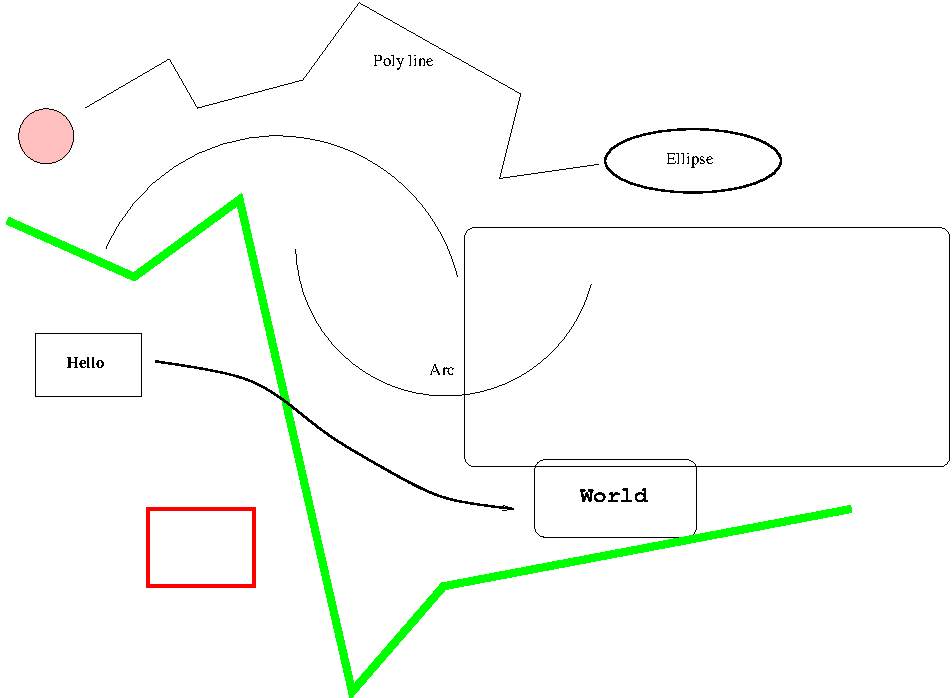
\includegraphics{figs/diagram.pdf}}
\caption{Example diagram drawn using \texttt{xfig}}
\label{xfig}
\end{figure}


\chapter{Evaluation}

\section{Printing and binding}

Use a ``duplex'' laser printer that can print on both sides to print
two copies of your dissertation. Then bind them, for example using the
comb binder in the Computer Laboratory Library.

\section{Further information}

See the Unix Tools notes at

\url{http://www.cl.cam.ac.uk/teaching/current-1/UnixTools/materials.html}


\chapter{Conclusion}

I hope that this rough guide to writing a dissertation is \LaTeX\ has
been helpful and saved you time.


%%%%%%%%%%%%%%%%%%%%%%%%%%%%%%%%%%%%%%%%%%%%%%%%%%%%%%%%%%%%%%%%%%%%%
% the bibliography
\addcontentsline{toc}{chapter}{Bibliography}
\bibliography{refs}

%%%%%%%%%%%%%%%%%%%%%%%%%%%%%%%%%%%%%%%%%%%%%%%%%%%%%%%%%%%%%%%%%%%%%
% the appendices
\appendix

\chapter{Latex source}

\section{diss.tex}
{\scriptsize\verbatiminput{diss.tex}}

\section{proposal.tex}
{\scriptsize\verbatiminput{proposal.tex}}

\chapter{Makefile}

\section{makefile}\label{makefile}
{\scriptsize\verbatiminput{makefile.txt}}

\section{refs.bib}
{\scriptsize\verbatiminput{refs.bib}}


\chapter{Project Proposal}

\setlength{\parskip}{0.75\baselineskip}

\maketitlep

% ******************************** Main Proposal *********************************

\chapter{Introduction}
\textit{In this chapter, I provide the motivation for this project and setup the problem I am solving. I also explain some key algorithms involved. Finally, I cover some related work.}

\section{Motivation}
	
 Transmission Control Protocol (TCP) is the protocol of choice in many data centers. However, it is very sensitive to losses (by design, as a mean for congestion control), which can degrade the performance within the data centers significantly \cite{zilberman2017has}. Various congestion control, avoidance and recovery mechanisms are thus of high importance in this field to minimise such loss rate. Still, not all TCP losses are born equal. For example, losses happening at the destination host's network interface card (NIC) are not an indication of congestion within the network. It is assumed that fast retransmission of such lost packets, from within the network, can increase the utilization of the network.
 
 In-network computing is an emerging research area in systems and networking, where applications traditionally running on the host are offloaded to the network hardware (e.g. switch, NIC). Examples of applications offloaded in the past include network functions (DNS server \cite{dns}), distributed systems functions such as consensus (P4xos \cite{p4xos}), various caching (netCache \cite{netCache}, netChain \cite{netChain}) and even a game (Tic-Tac-Toe). Key-Value Store (KVS) is also among the popular type of in-network applications. 
 
 Therefore, it is particularly interesting, and indeed challenging, to see how network-accelerated KVS concepts can be applied to TCP fast retransmit mechanism in order to improve cross-datacentre performance.
 
\section{Project Aims}
Fast retransmit is an enhancement to TCP that reduces the time a sender waits before retransmitting a lost segment. A TCP sender normally uses a simple timer to recognize lost segments. If an acknowledgement is not received for a particular segment within a specified time (a function of the estimated round-trip delay time), the sender will assume the segment was lost in the network, and will retransmit the segment.

Duplicate acknowledgement (DUP ACK) is the basis for the fast retransmit mechanism. After receiving a packet (e.g. with sequence number 1), the receiver sends an acknowledgement by adding 1 to the sequence number (i.e. acknowledgement number 2). This indicates to the sender that the receiver received the packet number 1 and it expects packet number 2. Suppose that three subsequent packets are lost. The next packets the receiver sees are packet numbers 5 and 6. After receiving packet number 5, the receiver sends an acknowledgement, but still only for sequence number 2. When the receiver receives packet number 6, it sends yet another acknowledgement value of 2. Duplicate acknowledgement occurs when the sender receives more than one acknowledgement with the same sequence number (2 in our example).

When a sender receives several DUP ACKs, it can be reasonably confident that the segment with the sequence number specified in the DUP ACK was dropped. A sender with fast retransmit will then retransmit this packet immediately without waiting for its timeout.

\begin{figure}[h]
	\centering
	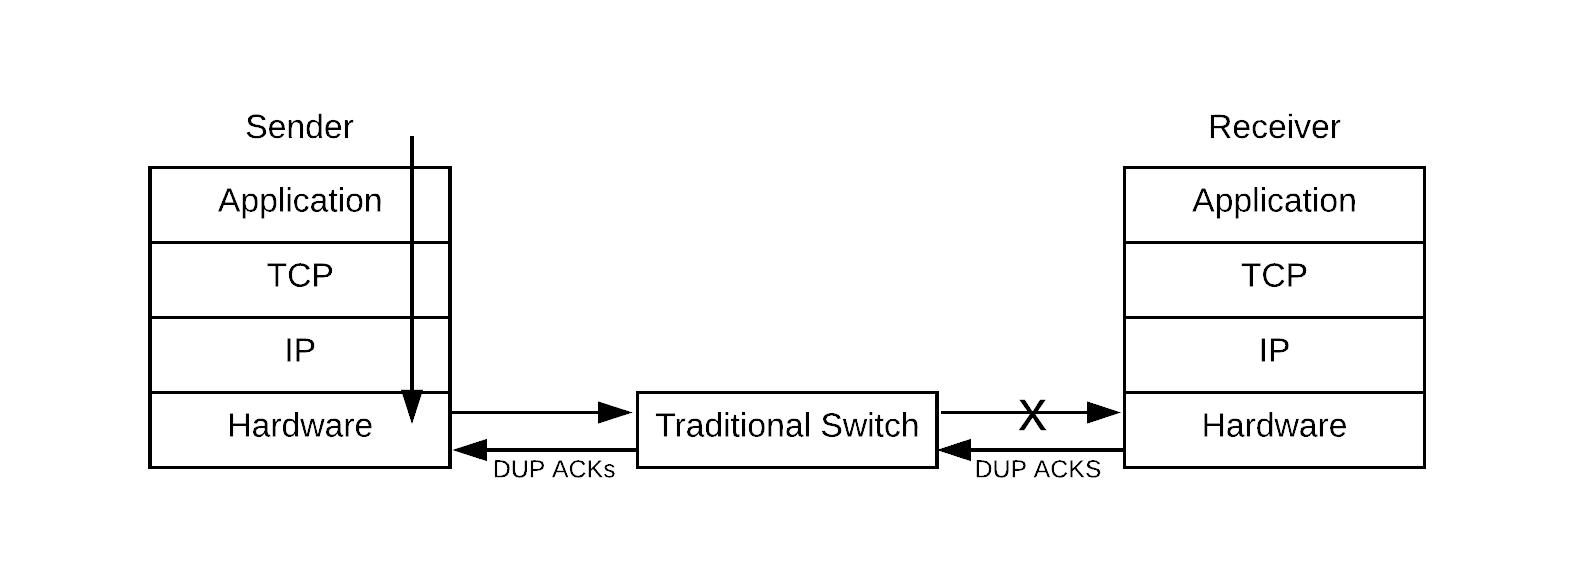
\includegraphics[width=\textwidth]{tradition-tcp.png}
	\caption{The standard convention of TCP handling.}
	\label{tradition-tcp}
\end{figure}

Currently, the DUP ACKs will traverse all the way back to the sender (\textbf{Figure \ref{tradition-tcp}}). The sender receives the DUP ACKs, then retransmits the packet with the next higher sequence number. 

\begin{figure}[h]
	\centering
	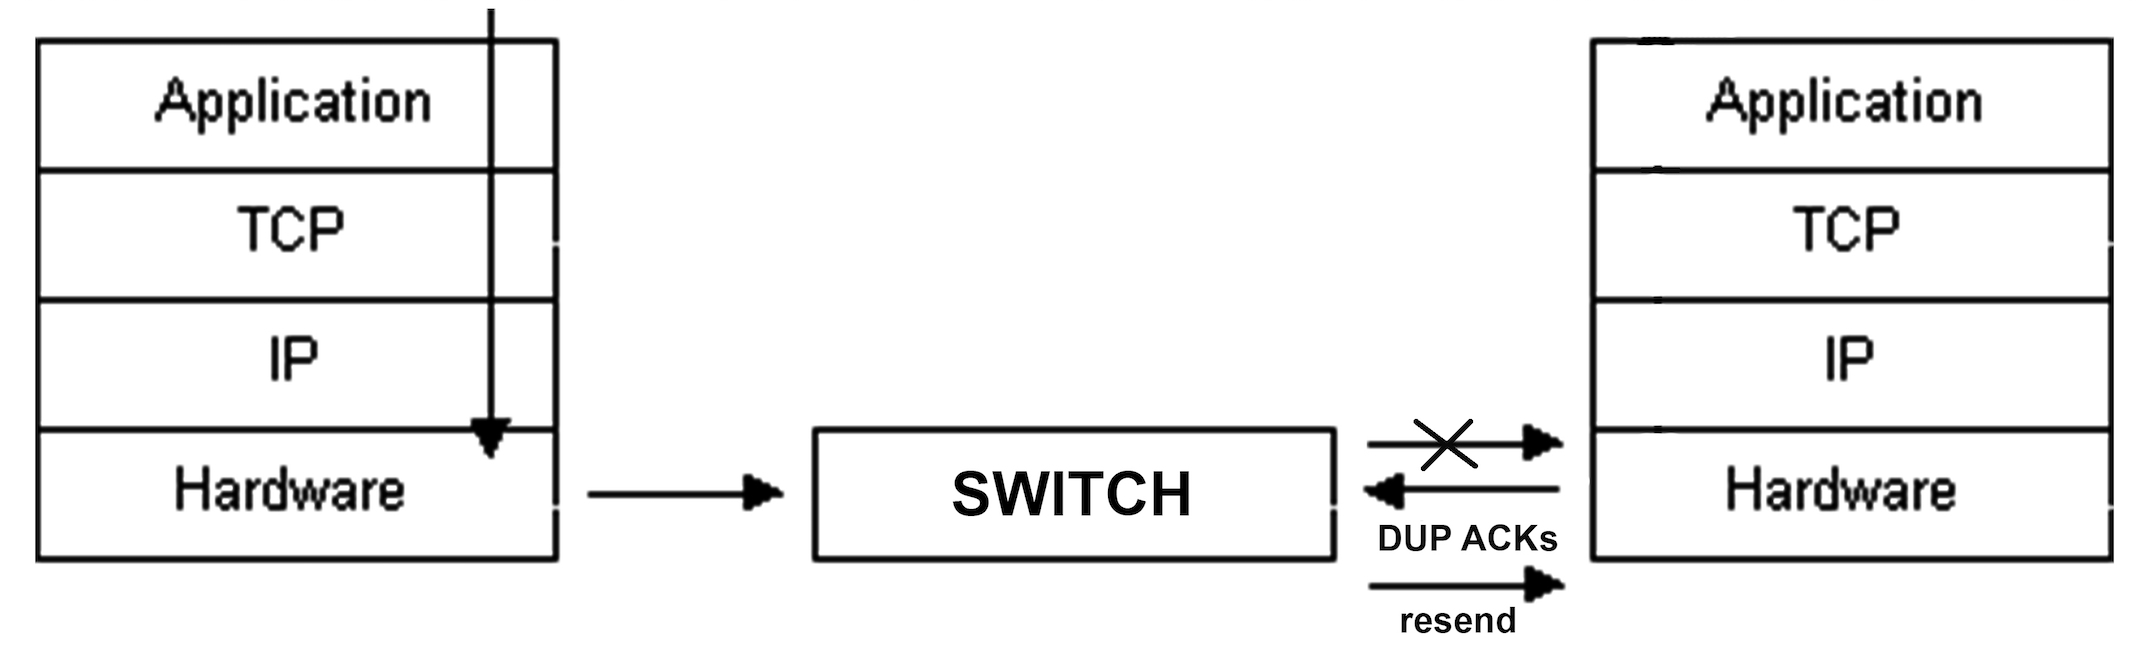
\includegraphics[width=\textwidth]{project-tcp.png}
	\caption{The proposed TCP handling.}
	\label{project-tcp}
\end{figure}

This project aims to design and implement a programmable switch that assists the TCP fast retransmit algorithm. The programmable switch will be able to retransmit the packets from within the network, instead of waiting for the DUP ACKs to get back to the host (\textbf{Figure \ref{project-tcp}}), thereby aims to reduce the response time to DUP ACKs and reduce unnecessary changes to the congestion window. The implementation will be based on the KVS concept, where the keys are the flow ID and the packet sequence number, and the value is the payload.

\section{Related Work}
	\subsection{TCP Congestion Control}
	One of the main aspects of TCP is congestion control, where a number of mechanisms are used to achieve high performance and avoid sending more data than the network is capable of forwarding, that is, to avoid causing network congestion. In particular, TCP uses a \textit{congestion avoidance} algorithm that includes various aspects of an additive increase/multiplicative decrease (AIMD) scheme, with other schemes such as \textit{slow start}, \textit{fast retransmit} and \textit{fast recovery} to achieve congestion avoidance. 
	
	The four intertwined algorithms are defined in more detail in RFC 5681\cite{rfc5681}. In this project, we are mostly interested in the \textit{fast retransmit} algorithm, which has been explained in the previous section.
	
	\subsection{Programmable Data Planes}
	The use of P4, netFPGA, etc.


\section*{\fontsize{18pt}{0.5}\selectfont Starting Point}

\subsection*{Platform \& Language}
This project will work mainly with a NetFPGA SUME board \cite{netfpgasume}, using P4 programming language. I will be using the P4-NetFPGA workflow, which provides infrastructure to compile P4 programs to NetFPGA \cite{fpga}. Apart from that, everything else will be built from scratch.

I have no prior experience with either NetFPGA or P4, but this will be mitigated through self-learning in which I will make use of the online tutorials, Google's resources and the P4 community documentation, as well as the experience of my supervisors. 

\subsection*{Computer Science Tripos}
The relevant Tripos courses that can serve as a starting point for this project are primarily: \emph{Computer Networking}, \emph{Principles of Communications} and \emph{ECAD and Architecture Practical Classes}. Since the courses are introductory, I will also consult Part III's \emph{High Performance Networking} course. I also plan to bridge any knowledge gap through extensive personal reading as well as help from my project supervisor.
\section*{\fontsize{18pt}{1}\selectfont Resources Required}

For this project I will be using my own computer, a 2017 MacBook Pro with a 2.3 GHz Intel Core i5 processor and 16 GB of RAM, that runs macOS Mojave. I accept full responsiblity for this machine, and I have made contingency plans to deal with hardware and/or software failures. Should that machine suddenly fail, I have another 16Gb of RAM computer with a 2.6 GHz Intel Core i7 processor that runs Ubuntu 18.04 LTS. If all else fails, I can continue to work on an MCS machine. Backups will be done weekly to Microsoft OneDrive and my external hardrive, and all my codes will be uploaded to GitHub for version control. 

For the hardware prototype, I will require a NetFPGA SUME board. I will need access to a machine that has the SUME installed, and a 10G NIC. These will be supplied by my supervisor. I will be using my own machine for development, with remote access to a server with the SUME board inside.

I will also require access to the lab network in order to \emph{ssh} to the server with the SUME board. Development on my machine will require VPN access, for using floating licenses of the development tools. Lastly, I will require a second server for testing some of the extensions of the project.
\section*{\fontsize{18pt}{1}\selectfont Work to be Done}

The main core component of the project is to be able to apply the KVS concept, where the sequence number and flow Id of a packet are the key and the packet is the value, to implement TCP fast recovery. In order to do that, the following sub-tasks must be done:

\begin{enumerate}
	
	\item First, since the project is done on NetFPGA using P4 programming language, both of which I am not familar with, I first have to study them thoroughly and be proficient working with the platform.
	
	\item I would also need to study and gain a better understanding of KVS applications, TCP congestion control and recovery mechanisms, as well as their use cases (e.g. High Frequency Trading, in-datacenter latency sensitive applications, etc.).
	
	\item The next stage will be to design the architecture for the application. This is a non-trivial process. Generally, it will be to try to map the application to a match-action pipeline.
	
	\item The fourth stage involves implementing the architecture in code. The program, which will be written in P4, will have the basic functionalities such as:
	\begin{itemize}
		\item A basic L3 switch function and TCP decoding (send TCP, read the flow information from the table/register)
		
		\item Matching packets to a "\emph{key}" (its flow Id):
			\begin{itemize}
				\item If the key is of a new packet, store it (SET()).
				\item If the key is of a DUP ACK, read the packet and re-send (GET()).
				\item If the number of DUP ACKs is greater than $N$, do not resend. Instead, forward to host as the standard convention of handling TCP.
				\item Do not resend if the flow Id is not in a "selected" table. In other words, use the KVS only if the flow Id matches a predefined set of flow Ids, or a different predefined rule by the user.
			\end{itemize}		
	
	\end{itemize}
	
	\item \textbf{The simulation stage:} perform functionality test by simulating the program using bmv2 or Xilinx simulators to ensure correctness. 
	
	\item After it runs smoothly in the software, it will then be compiled to the hardware. Ensure that the basic functionalities mentioned above work in hardware.
	
	\item \textbf{The hardware stage:} demonstrate interoperability with a software-based client/application.
	
	Possibly, I will implement a drop $1:N$ packets at the server to force DUP ACKs, and I will also be using a synthetic benchmark such as \emph{multilate} \cite{multilate} -- a memcached benchmark -- or OSNT \cite{OSNT} as the applications on top of the network. The criterion to evaluate the performance is the flow completion time. There is no intention to use network simulators such as ns2, omnet++, etc. This is outside the scope of this project.
	
	The aim for this stage is to get a working prototype in hardware that supports a single flow and single packet size, and evaluate on its performance.
	
	\item Once the prototype is up and working, I need to implement further extensions to allows the prototype to support a variety of parameters/conditions (which will be discussed in \textbf{Possible Extensions} section).
		
\end{enumerate}

\section*{\fontsize{18pt}{1}\selectfont Success Criteria}

This project will be deemed a success if I managed to study and design an architecture for the application, as well as succeeded to implement that design. More concretely:

\begin{enumerate}
	\item I have an implementation of the application written in P4.
	
	\item The implementation works in simulation (using bmv2/Xilinx simulators).
	
	\item I have a working prototype. In other words, my design runs on the hardware.
	
	\item I am able to demonstrate interoperability with a software-based client/application.
	
	\item I can provide a performance evaluation of the design.
\end{enumerate}
\section*{\fontsize{18pt}{1}\selectfont Possible Extensions}

If the core parts of the project are successful and completed within a reasonable time, I shall then try to investigate and implement further extensions. Some possible options are:

\begin{enumerate}
	\item Supporting more than a single flow, and supporting the configuration of flows to monitor (\& retransmit)
	
	\item Supporting different packet sizes (depends on workflow limitations).
	
	\item Sending a notification to the source if multiple retransmits fail.
	
	\item Adaptively installing and deleting from the list of flows to monitor.
	
	\item A performance evaluation comparison to existing TCP recovery mechanisms.
\end{enumerate}
\section*{\fontsize{18pt}{1}\selectfont Timetable}

The schedule is broken into 15 2-week periods, with the first period starting on 19/10/2018.

\begin{enumerate}
	%1
	\item \textbf{Michaelmas weeks 2--4 [19/10--5/11]:} Preparatory reading on the P4 programming language and setting up the NetFPGA platform. Going through the tutorials and experimenting with some examples. Study TCP congestion control and recovery mechanisms beyond the material taught in \emph{Computer Networking} and \emph{Principles of Communications} courses.
	
	%2
	\item \textbf{Michaelmas weeks 5--6 [6/11--19/11]:} Design the architecture: mapping the application to a match-action pipeline.
	\\
	\textbf{\underline{Milestone:} Understand the application architecture. Be able to map the application to a match-action pipeline.}
	
	%3
	\item \textbf{Michaelmas weeks 7--8 [20/11--28/11]:} Start implementing of the design by writing the basic code. 
	
	%4
	\item \textbf{Michaelmas vacation weeks 1--2 [30/11--12/12]:} Simulate the application using bmv2/Xilinx simulators. 
	\\
	\textbf{\underline{Milestone:} Basic design written in P4 working in simulation, with minimal bugs left.} .
	
	%5
	\item \textbf{Michaelmas vacation weeks 3--4 [13/12--26/12]:} Start to implement the working code into hardware. Write a hardware-test program (Python-based). 
	
	%6
	\item \textbf{Michaelmas vacation weeks 5--7 [27/12--16/1]:} Demonstrate interoperability with a software-based client/application. Start writing the progress report.
	\\
	\textbf{\underline{Milestone:} Have the application working in hardware, a completed progress report and a presentation for demonstration purposes.}
	
	%7
	\item \textbf{Lent weeks 1--2 [17/1--30/1]:} Work on the design's performance testing and evaluation.
	
	%8
	\item \textbf{Lent weeks 3--4 [31/1--13/2]:} Continue working on testing and evaluation of the design.
	\\
	\textbf{\underline{Milestone:} The project is finished and meets the success criteria.}
	
	%9
	\item \textbf{Lent weeks 5--6 [14/2--27/2]:} Start working on extensions, based on project's progress.
	\\
	\textbf{\underline{Milestone:} The prototype continues to work well with the extensions implemented.}
	
	%10
	\item \textbf{Lent weeks 7--8 [28/2--13/3]:} Possible overflow from the previous weeks. Clean up codes and repository. Start writing dissertation main chapters.
	\\
	\textbf{\underline{Milestone:} Completed working prototype with core components and extensions in place. First draft of dissertation}
	
	%11
	%12	
	%13
	\item \textbf{Easter vacation:} Continue writing dissertation. Review cycles and corrections to dissertation towards the end of the vacation.
	
	%14
	\item \textbf{Easter weeks 1--2 [25/4--8/5]:}  Completed dissertation. Proof reading and then an early submission so as to concentrate on examination revision.
	
	%15
	\item \textbf{Easter weeks 3 [9/5--17/5]:} Buffer week.
\end{enumerate}


\end{document}
